\documentclass[11pt]{article}
\usepackage[margin=0.85in]{geometry}
\usepackage[T1]{fontenc}
\usepackage{lmodern}
\usepackage{amsmath,amssymb,booktabs,array,tabularx,xcolor,graphicx}
\usepackage[hyphens]{url}
\usepackage[colorlinks=true,linkcolor=blue!45!black,citecolor=blue!45!black,urlcolor=blue!45!black]{hyperref}
\newcommand{\file}[1]{\nolinkurl{#1}}
\newcommand{\eps}{\varepsilon}
\newcolumntype{L}[1]{>{\raggedright\arraybackslash}p{#1}}
\setlength{\parskip}{4pt}
\setlength{\parindent}{0pt}
\setlength{\emergencystretch}{2em}
\renewcommand{\arraystretch}{1.13}
\hypersetup{pdftitle={An Allocation Framework for Opaque Quantum Circuits},pdfauthor={DuQuantum BlueQubit Team}}
\title{\vspace{-1.1cm}An Allocation Framework for Opaque Quantum Circuits\\\large Pre-Challenge Design, Empirical Tests, and Revision}
\author{DuQuantum BlueQubit Team}
\date{Evidence snapshot: October 24, 2026}

\begin{document}
\maketitle
\vspace{-1em}
\begin{abstract}
We developed a framework before the challenge for allocating limited computation across matrix product state and Pauli-path approximations, then revised it using sample calibration, native-backend diagnostics, submission feedback, and failed refinements. Its contribution is a reproducible decision protocol linking precision trends, score-relevant vector shape, representation choice, and resource accounting. Exact reuse supplied G1's reported 300/300; Kevin's G3 threshold refinement accompanied an increase from 534/800 to 773/800; and a later repository note reports 579/600 for a mixed-precision G2 submission, with its account and row provenance still unresolved. G4's accepted zero score and negative extrapolation tests supplied evidence for changing the protocol. These account-specific outcomes support a case study of empirical framework development; they do not establish a controlled performance advantage over alternative allocation policies. Execution is paused, and the write-up uses saved evidence only.
\end{abstract}

\section{The objective was the shape of an observable vector}
Each published identifier \file{Duke_<problem>_<q>} denotes a separate program, not another measurement on a shared simulated state. For its circuit $U_{c,q}$, the target is
\begin{equation}
 F^*_{c,q}=\langle 0^{n_c}|U_{c,q}^{\dagger}Z_qU_{c,q}|0^{n_c}\rangle.
\end{equation}
The SDK's Pauli string places qubit zero at the right. Correct ID coverage, observable construction, and ordering were prerequisites to every numerical comparison. The public samples contain 4, 16, and 30 IDs; G1--G4 contain 30, 36, 36, and 38. Only the samples expose circuit QASM.\cite{challenge}

The two approximation families compress different objects. MPS represents the state by a chain of tensors; its bond dimension $\chi$ limits the Schmidt rank retained across each cut. Increasing $\chi$ allows more entanglement to be represented but does not by itself certify the target observable. PPS propagates an observable as a sum $O=\sum_P c_P P$ of Pauli strings. Clifford conjugation maps a Pauli string to another Pauli string, whereas non-Clifford gates can branch that expansion. Removing small coefficients controls its size while changing cancellations and the final expectation. This explains our chain-versus-mostly-Clifford method prior, and why a PPS coefficient threshold is not a final-observable error bound.\cite{design,kevin}

The retained challenge rules award a problem of weight $w_c$ the score
\begin{equation}
 S_c=w_c\bigl[\max(0,\rho(\widehat{\mathbf F}_c,\mathbf F_c^*))\bigr]^2,
 \qquad
 \rho(\mathbf x,\mathbf y)=
 \frac{\mathbf x_0^\top\mathbf y_0}{\|\mathbf x_0\|_2\|\mathbf y_0\|_2},
 \label{eq:score}
\end{equation}
where $\mathbf x_0=\mathbf x-\bar x\mathbf1$ and similarly for $\mathbf y_0$; constant predictions score zero. Weights are 100 for each sample and 300, 600, 800, and 1000 for G1--G4.\cite{rules}

This objective rewards positively correlated \emph{shape}. A common offset or positive scale leaves Pearson correlation unchanged; a sign reversal does not. Ordering is informative but insufficient: Pearson correlation also depends on relative spacings. For nonconstant matched vectors, fitting $a=(\mathbf x_0^\top\mathbf y_0)/(\mathbf x_0^\top\mathbf x_0)$ gives
\begin{equation}
 \frac{\|\mathbf y_0-a\mathbf x_0\|_2^2}{\|\mathbf y_0\|_2^2}=1-\rho^2.
 \label{eq:residual}
\end{equation}
We therefore inspected signed correlation, affine residuals, zero counts, and order changes alongside pointwise increments. Equation~\eqref{eq:residual} describes agreement between approximations, not their error against hidden truth. Negative slopes still matter, two nonconstant points always have $|\rho|=1$, and weak centered signals can make small absolute errors consequential.

\newpage
\section{The framework preceded the results}
The team prepared the version-zero design before the problem set was released. Its document is dated October 22, and Git commit \file{8fac5d9} preserves it on October 23 at 23:09 EDT, before the stated October 24 kickoff. The filename calls it v0, although its internal title says Version 1.0. It already proposed MPS/PPS precision sweeps, vector-shape diagnostics, transpilation sensitivity, adaptive resource allocation, and sample-validated extrapolation or fusion. It explicitly described these as unvalidated proposals.\cite{design}

Our research sequence was therefore \emph{design, implementation, observation, revision}. The current framework develops that design; it is not a claim that its concepts were invented after seeing the scores. Nor was v0 a formal preregistration: it contained provisional assumptions, including two samples and an illustrative CSV schema, which the released kit replaced. Table~\ref{tab:evolution} records substantive changes in how the proposed ideas were applied.

\begin{table}[h!]
\small
\begin{tabularx}{\textwidth}{@{}L{1.35in}XX@{}}
\toprule
Initial design & Empirical finding & Revision supported by evidence \\
\midrule
Compare MPS and PPS precision sequences & G4 had sensitive, nonuniform MPS trends and uninformative PPS zeros. & Require within-method trends and informative corroboration; agreement alone cannot close the question. \\
Test transpilation sensitivity & Native PPS levels 2/3 returned zero on a known S3 test; 0/1 recovered signal. & Resolve representation failure before tightening precision. \\
Allocate by expected benefit per cost & Easy G2 endpoints concealed transition sensitivity; quotes differed from measured runtime. & Predeclare a decision-changing panel and separate feasibility, numerical sensitivity, and settled cost. \\
Validate extrapolation and fusion & Held-out extrapolation worsened both tested windows; fusion showed no gain. & Retain direct estimates and disable unsupported transformations. \\
Refine a complete baseline & A later G2 report uses 23 GPU $\chi=512$ rows with 13 $\chi=64$ rows. & Treat selective precision as a candidate extension requiring row provenance and evaluation; it is not yet supported by the coherent-cohort exporter. \\
\bottomrule
\end{tabularx}
\caption{Evolution of pre-existing hypotheses into operational rules. The evidence and its chronology are retained in the decision ledger.}
\label{tab:evolution}
\end{table}

\subsection{A decision protocol with explicit evidence gates}
Let $E_t$ contain the saved vectors, precision settings, jobs, costs, and attributed feedback available at time $t$. A proposed experiment $a$ specifies an ID, simulator, representation, precision, and hardware. Before executing it, record the decision it tests and how contrasting outcomes would change the next action. If both outcomes lead to the same action, its immediate decision value is low. Reuse existing evidence before admitting another computation.

The protocol has four gates: \textbf{representation} asks whether the chosen method resolves useful signal; \textbf{precision} examines signed within-method changes and independent agreement; \textbf{shape} measures changes that survive removal of a common offset and positive scale; and \textbf{resources} checks dollar commitments, elapsed time, quotas, and completion risk. No diagnostic substitutes for the others. A completed expensive job may add little decision information; a cheap sign-sensitive row may change the allocation.

For a matched pair of centered profiles, define $r=\mathbf y_0-a\mathbf x_0$ using the fitted slope from Eq.~\eqref{eq:residual}. The influence $I_q=r_q^2/\|r\|_2^2$, when defined, ranks where the observed shape discrepancy is concentrated. It is a way to select complementary tests, not a probability that row $q$ is wrong. Retain separated interior and sign-sensitive rows so a panel does not depend entirely on a few dominant coordinates.

The resulting contribution is an inspectable allocation framework for opaque circuits under a correlation objective: its experiments can be traced from a question to a receipt to a revised decision. MPS, PPS, residual analysis, and adaptive allocation are established ideas. Our claimed contribution is their explicit integration and empirical refinement in this setting; field-wide originality or general superiority would require a literature comparison and prospective evaluation beyond this case study.

\newpage
\section{Results and the evidence supporting them}
Table~\ref{tab:results} records actual submission outcomes without treating teammate reports as browser observations. ``Original'' denotes the original submitting account; ``Kevin'' denotes his imported record. The ledger retains file hashes and row provenance.\cite{ledger,kevin}

\begin{table}[h!]
\centering
\small
\begin{tabularx}{\textwidth}{@{}L{0.66in}L{2.12in}L{0.75in}X@{}}
\toprule
Problem & Retained method or artifact & Score & Evidence and status \\
\midrule
S1--S3 & S1/S2 local exact; S3 local PPS, $\eps=0.01$ & 100/100 each & Original; browser-observed submissions. \\
G1 & Exact CPU, 30 rows & 300/300 & Kevin; teammate-reported. Original account separately confirmed submission; its score is unknown. \\
G2 & CPU MPS, $\chi=32$ & 342/600 & Original; user-reported first attempt, 3.48-hour time penalty. \\
G2 & CPU MPS, $\chi=128$ & 498/600 & Kevin; teammate-reported, with distinct verified CSV and job provenance. \\
G3 & Native PPS, level 1, $\eps=0.001$ & 534/800 & Kevin; teammate-reported submitted v2. \\
G3 & Native PPS, level 1, $\eps=0.0003$ & \textbf{773/800} & Kevin; teammate-reported submitted v3. \\
G4 & CPU MPS, $\chi=32$ & 0/1000 & User-reported accepted result; account and attempt unknown. \\
G2 & Mixed $\chi=512/64$ vector & 579/600 & Repository text claim; user confirmed submission. Account, attempt, penalty, and row provenance unresolved. \\
\bottomrule
\end{tabularx}
\caption{Recorded outcomes as of the evidence snapshot. Displayed scores may be rounded. The 579/600 claim has weaker provenance than Kevin's attributed receipts; rows from different accounts do not establish one account's total.}
\label{tab:results}
\end{table}

An older receipt attributed G2's 498/600 to the original $\chi=32$ bytes. Kevin's later record assigns it to his distinct $\chi=128$ file. That older attribution remains disputed; a time penalty cannot reconcile different score/file claims. The 342-to-498 comparison is consequently not a controlled same-account precision experiment. The original G3 $\eps=0.001$ candidate contains the same 36 numerical values as Kevin's v2, with different CSV serialization, but has no original-account submission score.\cite{ledger}

\subsection*{Calibration supplied a prior, not a hidden-circuit guarantee}
Public circuits permitted comparison with independently computed exact values. A stricter local calibration selected S1 MPS $\chi=8$, S2 MPS $\chi=128$, and S3 PPS $\eps=0.001$, with maximum errors approximately $2.7\times10^{-15}$, $0.00329$, and $0.00653$. Those settings differ from the actual sample uploads in Table~\ref{tab:results}; a rounded 100/100 did not certify pointwise exactness.\cite{calibration}

For G2's one-dimensional Haar chain, Kevin additionally built a 24-qubit proxy at the graded chain's depth. Its MPS squared correlation rose from about 0.997 at $\chi=64$ to 1.000 at $\chi=128$; PPS at $\eps=0.001$ reached about 0.974. For G3's mostly-Clifford grid, the structurally related S3 favored PPS over MPS. These tests supported \emph{which family to refine}. They did not forecast the graded scores, and no equally matched public family established a reliable prior for G4.\cite{kevin}

\newpage
\section{Decisions behind the highest documented scores}
\subsection{G1: reuse an exact anchor}
G1's 30-qubit programs fitted the available exact CPU route. Kevin's complete vector was reported as 300/300 and retained per-job evidence. Importing the verified vector avoided 30 duplicate simulations. This was a direct allocation improvement: exact evidence already existed, so repeating its production offered no numerical benefit. Its reuse did not transfer Kevin's score to the original account.\cite{kevin,ledger}

\subsection{G2: use chain structure, then stop for resources honestly}
MPS was selected for G2 because both the sample chain and depth-matched proxy favored it. Kevin's submitted $\chi=128$ vector scored a reported 498/600 with account-attributed row receipts. Its residual uncertainty remained visible: a partial $\chi=256$ follow-up moved q2 from approximately 0.916 to 0.854. Kevin recorded quotes near \$10.88 and seven hours for an interior job, with a roughly \$360 full-run estimate. These were estimates, not incurred charges. Stopping that refinement was a resource decision, not convergence evidence.\cite{kevin,ledger}

Later original-account analysis exposed another allocation trap. Three rows, q0/q18/q35, gave $\rho\approx0.99999965$ between $\chi=16$ and 32 because saturated endpoints dominated the panel. Subsequent $\chi=64$ checks moved q9 from 0.494442 to 0.301455 and q31 from 0.551690 to 0.416197. These transition rows supplied sensitivity evidence missed by the endpoints. This lesson improves future diagnostic selection; it was not the cause of Kevin's earlier 498/600.\cite{decisions,ledger}

A later repository note, committed as \file{030518f}, reports \textbf{579/600} for a complete $\chi=64$ baseline with 23 completed GPU $\chi=512$ results substituted and the other 13 baseline values retained. The user confirmed that CSV was submitted. This is the highest reported G2 score in the repository, but the account, attempt, penalty, and row-to-job mapping remain unknown; the website score has not been independently checked. The strategy illustrates selective expenditure on finer approximations while preserving complete coverage. The record does not show why those particular 23 IDs were selected or whether completion order determined the subset, so it cannot validate an optimal allocation rule or a controlled 498-to-579 gain.\cite{ledger}

\subsection{G3: resolve representation failure before tightening precision}
PPS performance depended on a native transpilation option, not only its truncation threshold. At $\eps=0.01$, the known sample \file{Duke_S3_1} returned approximately $-0.595$ and $-0.580$ at native levels 0 and 1, versus an exact value near $-0.538$; levels 2 and 3 returned zero. Stored-ID and uploaded-QASM tests did not remove the behavior. Native default level 2 also yielded constant-zero G3 results in the recorded tests.\cite{kevin}

Selecting level 1 addressed that empirical failure before increasing precision. Kevin's interpretation is that lighter transpilation better preserves useful Clifford structure; the service's internal mechanism was not independently established. The evidence supports the choice on these circuits, not a universal claim about transpilation levels.

\newpage
\subsection{G3: refine the threshold while holding representation fixed}
At fixed level 1, the complete G3 profiles then changed as follows:
\begin{center}
\begin{tabular}{@{}lrrl@{}}
\toprule
PPS threshold & Zero rows & Submitted score & Comparison with preceding profile \\
\midrule
$0.01$ & 33/36 & Not submitted & --- \\
$0.001$ & 9/36 & 534/800 & $\rho^2\approx0.00$ \\
$0.0003$ & 3/36 & 773/800 & $\rho^2\approx0.80$ \\
\bottomrule
\end{tabular}
\end{center}

The \textbf{239-point increase} is the strongest retained graded improvement under a controlled threshold change on Kevin's submission path. It is consistent with resolving the small, shape-sensitive G3 values. Fewer exact zeros and stronger inter-threshold agreement supported refinement; neither predicted 773 in advance nor certified convergence. Raw simulator values were retained without fitting.\cite{kevin,ledger}

\begin{figure}[h!]
\centering
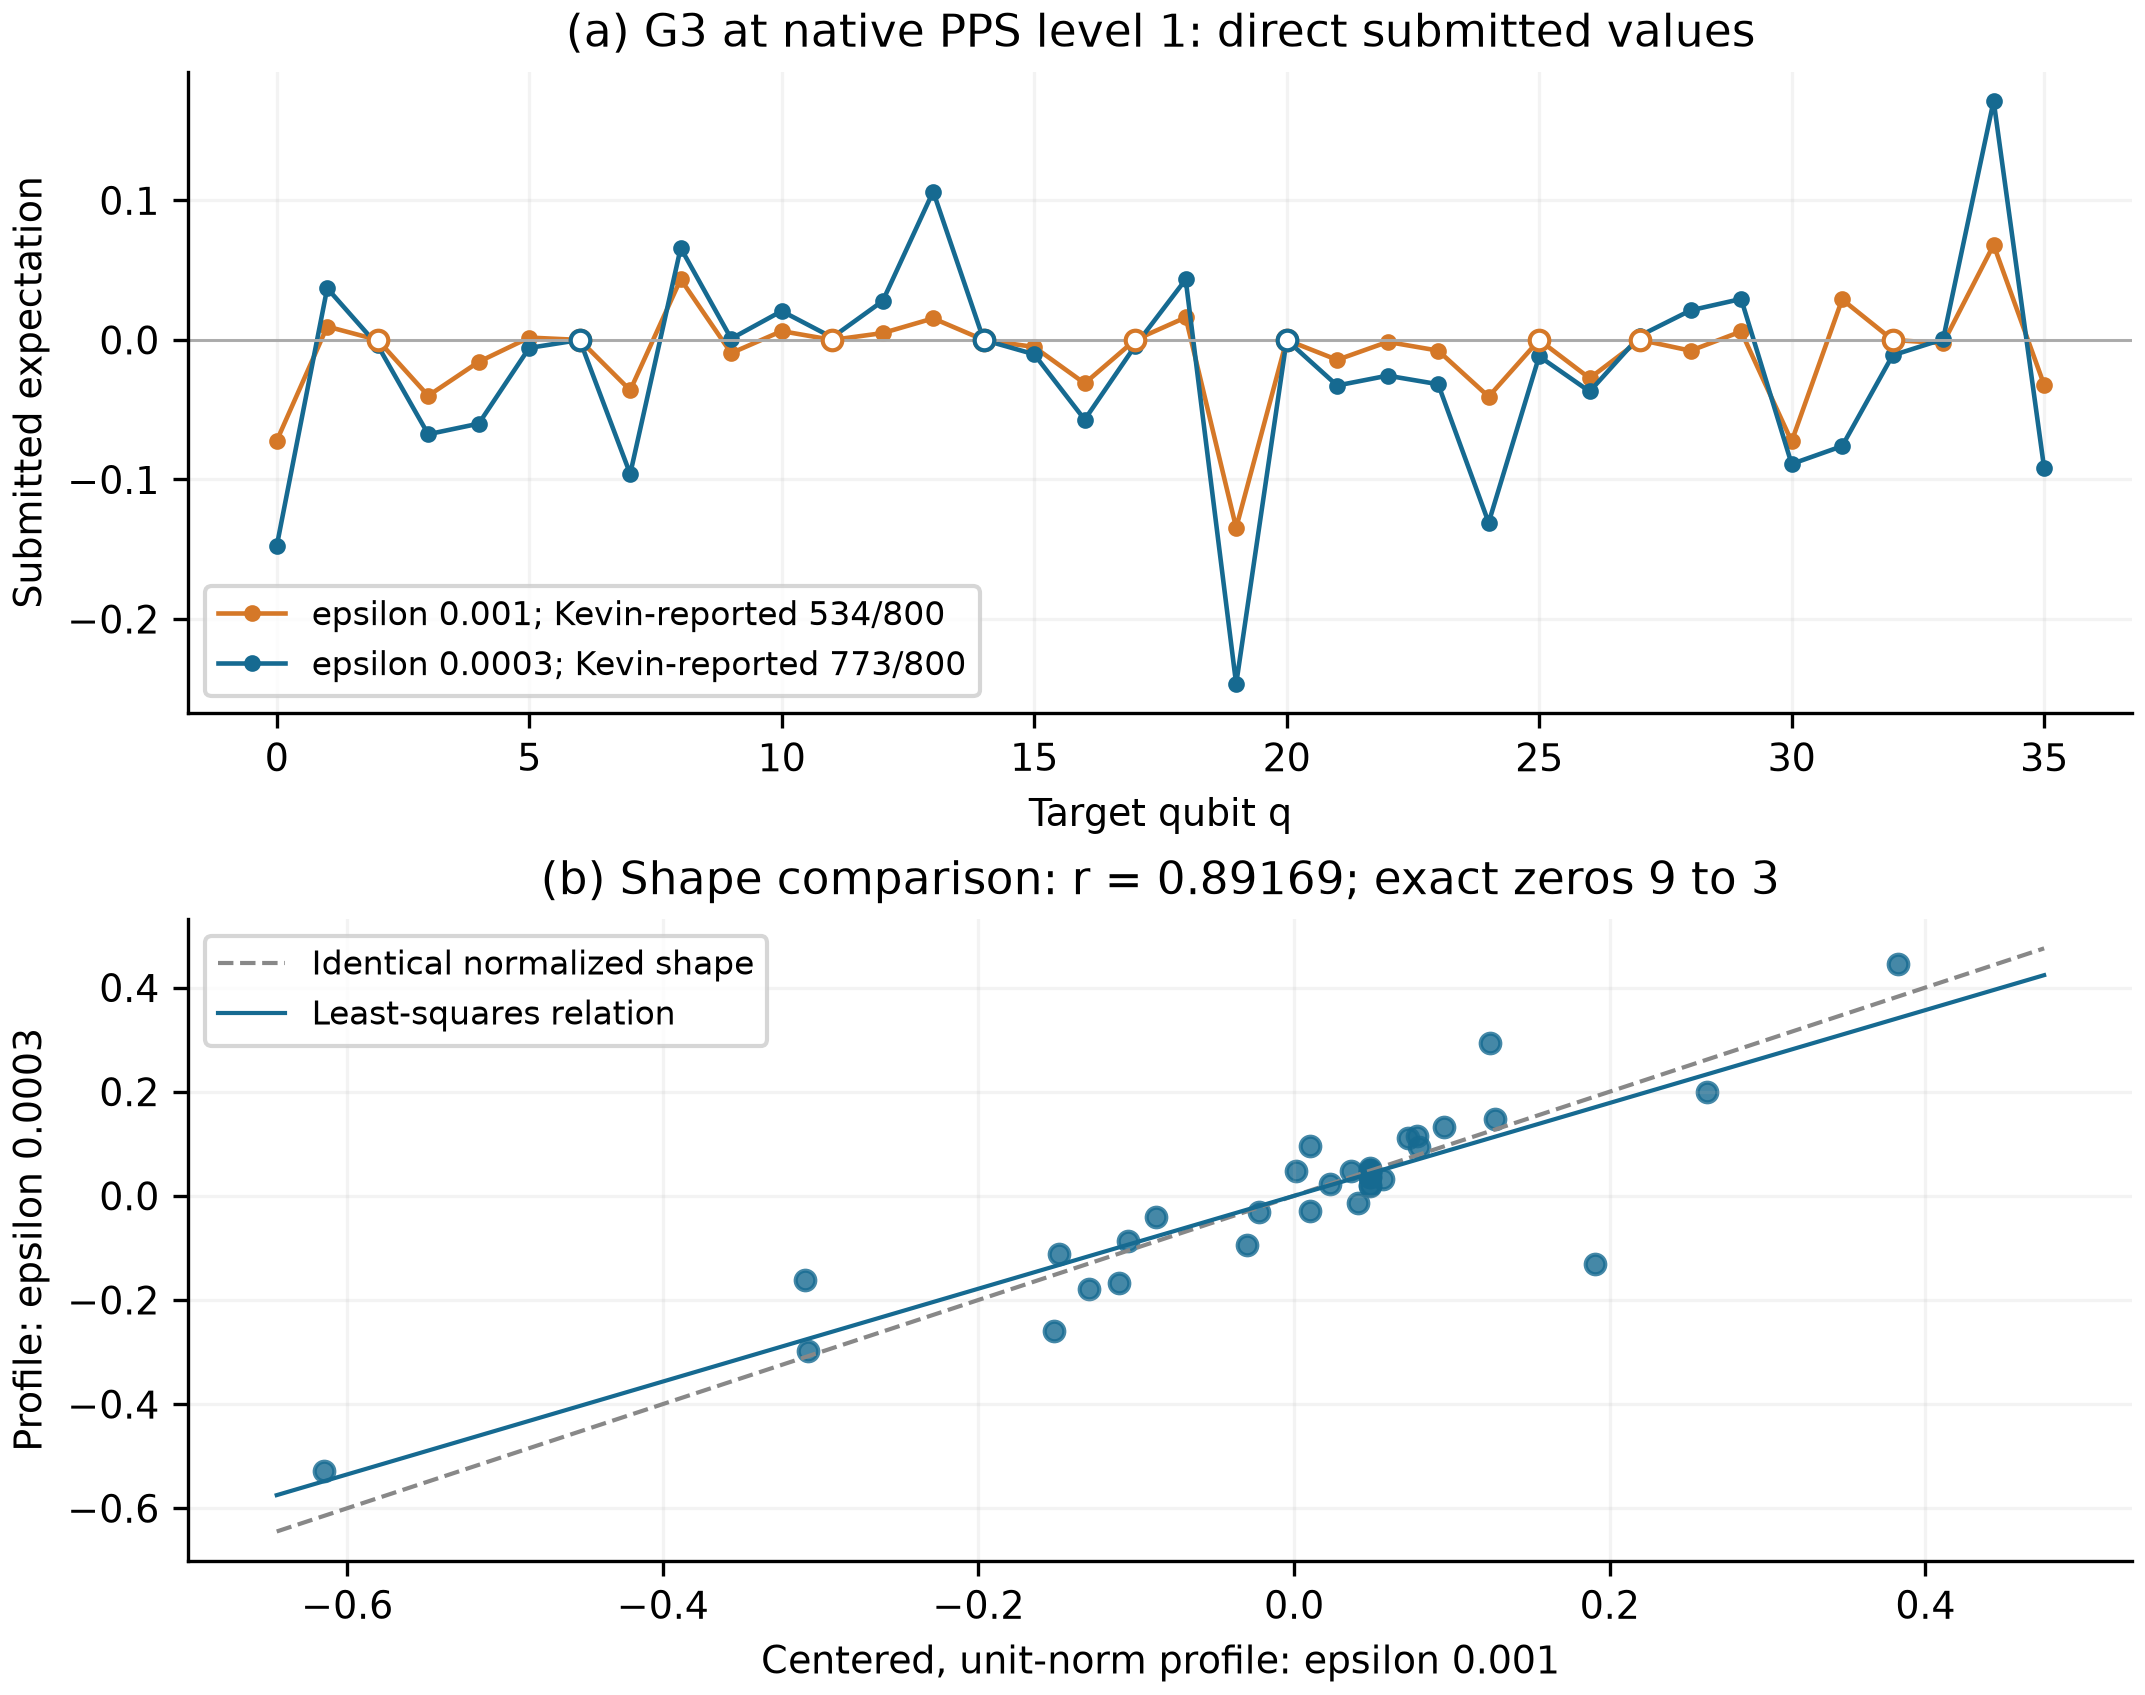
\includegraphics[width=\textwidth,height=3.8in,keepaspectratio]{figures/g3_precision.png}
\caption{Kevin's two submitted G3 vectors: raw expectations and centered, normalized profiles. Normalization means $(\mathbf v-\bar v\mathbf1)/\|\mathbf v-\bar v\mathbf1\|_2$ and is used only for display. The vectors have $\rho=0.89169$ and $\rho^2=0.79511$; exact zeros fall from nine to three. Scores 534/800 and 773/800 are Kevin-reported. No hidden reference is used in either plot, so this comparison describes shape evolution without establishing hidden error or score causality.}
\label{fig:g3}
\end{figure}

\newpage
\section{Failures were evidence about where to stop}
\subsection{G4: local contraction did not generalize}
The complete G4 $\chi=32$ artifact passed local format and provenance checks but received an accepted, user-reported 0/1000. On ten matched $\chi=16/32$ rows, $\rho=0.85912$, affine residual energy was 26.19\%, and 12 of 45 pairs reversed order. q0/q4 contributed 60.49\% of that subset's residual energy, motivating targeted checks. Residual influence located disagreement between approximations, not hidden error.\cite{g4,ledger}

\begin{table}[h!]
\centering
\small
\begin{tabularx}{\textwidth}{@{}lrrrX@{}}
\toprule
Row & $\chi=16$ & $\chi=32$ & $\chi=64$ & Diagnostic conclusion \\
\midrule
q0 & 0.558910 & 0.270272 & 0.097787 & Increments shrink but remain substantial. \\
q4 & $-0.005732$ & 0.331990 & 0.493042 & Increments shrink in the opposite direction. \\
q1 & 0.135555 & $-0.053917$ & 0.007232 & Direction reverses; signs remain sensitive. \\
q19 & 0.362228 & 0.288101 & 0.084401 & Latest increment grows about 2.75-fold. \\
\bottomrule
\end{tabularx}
\caption{Four completed CPU diagnostics, not a complete $\chi=64$ candidate. They refute extrapolating the first two rows' contraction to the whole problem.}
\end{table}

All four $\chi=64$ jobs completed within their diagnostic elapsed thresholds and recorded zero charge. Feasibility on these IDs did not justify a 38-row commitment. An independent-family q4 check also remained uninformative: native level-1 PPS returned zero at both $\eps=0.001$ and 0.0001 while compute rose from 5.350 to 178.913 seconds, a 33.4-fold increase. Matching zeros did not establish the answer; the result argued against blind threshold escalation.\cite{decisions,gpu}

\subsection{Partial G3 work did not produce the best documented result}
The original-account $\eps=0.0005$ G3 panel motivated a bounded continuation in an earlier review. That later cohort was stopped when the user changed direction, with 9 of 36 rows completed and two jobs canceled. The retained stop snapshot records no owned running jobs and known terminal costs; it does not represent a complete candidate or submission.\cite{stop} This work did not cause Kevin's 773/800: that finer, complete $\eps=0.0003$ vector was already available in his separate records. Reusing it supersedes the rationale for duplicating a coarser full cohort.\cite{ledger,decisions}

\subsection{Extrapolation and fusion were rejected rather than assumed helpful}
Offline geometric/Aitken extrapolation on saved S2 precision histories worsened held-out next-level MAE in both evaluated windows: 0.04676 versus 0.04447, and 0.01344 versus 0.00955 for the direct estimate. The second window also lost about 3.86 points against exact values. Leave-one-circuit-family-out fusion showed no held-out gain. Both remained disabled.\cite{rejections,calibration}

The useful standard was evidence that an added transformation improved a held-out comparison. A smooth sequence, averaging two biased methods, or a higher nominal precision alone could not satisfy it. Whole-problem scores were never converted into per-row corrections.

\newpage
\section{Resources should buy useful precision}
\subsection{Hardware acceleration is conditional on the workload}
A matched G4 q0 trial at $\chi=32$ produced CPU/GPU values differing by only $6.63\times10^{-12}$. GPU compute time was 24.189 seconds versus CPU's 48.593, but elapsed time fell only from 55.055 to 44.804 seconds: a 10.25-second saving for \$0.20 rather than the CPU receipt's \$0. The comparison established consistency and timing at one setting, not better mathematical precision. CPU $\chi=64$ subsequently fitted its diagnostic limits, so another same-precision GPU timing repeat was deferred.\cite{gpu}

The supplied paper motivates testing GPU routes when they make finer approximations attainable. It also cautions against universal speedup claims: in its examples, 96-qubit QFT at $\chi=64$ favored CPU, whereas a large kicked-Ising PPS workload strongly favored GPU. Its PPS error curve was nonmonotonic. These workload-specific observations do not certify hidden Duke values, and its target-bit overlap metric is not state fidelity or Pearson score.\cite{paper}

The campaign obtained dated GPU quotes, including PPS estimates of 0.1 seconds, but those are not measured runtime. No high-$\chi$ GPU or GPU-PPS score improvement is claimed. Qiskit, Quantum Rings, Julia, and related local alternatives require gates or QASM; installing another simulator cannot replace the hidden circuits' missing input.\cite{gpu,decisions}

\subsection{Cost evidence and stopping conditions remain separate}
The operating budget was \$30, with a \$27 planning ceiling. Admission considered recorded charges and outstanding/new quoted commitments, not only settled spend. Samples recorded zero cloud charges; Kevin's submitted results report zero total credits; the original-account stop snapshot records \$0.20 in known charges, consistent with the matched GPU trial. These account-specific records are not a complete final billing statement or a promise that future CPU work is free. Quotes, elapsed cancellation thresholds, quota use, terminal status, and billed cost answer different questions.\cite{ledger,gpu,workflow,stop}

The saved workflow has status \file{PAUSED_NO_NEW_RUNS}. It is the current revision of the pre-challenge design, informed by observations and made explicit in this synthesis. It does not imply that every experiment followed an unchanged plan. If execution is explicitly resumed, its decision procedure is:
\begin{enumerate}
\setlength{\itemsep}{2pt}
\item \textbf{Reuse complete evidence.} Check existing vectors, exact options, receipts, account attribution and unresolved jobs before proposing computation.
\item \textbf{Choose a decision-changing test.} Separate representation from precision; select informative transition, sign-sensitive or interior rows rather than a fixed quota of easy pilots.
\item \textbf{Review sensitivity and shape together.} Preserve signed changes, residuals, zeros and order; seek informative independent corroboration without interpreting agreement as truth.
\item \textbf{Choose hardware for useful precision.} Admit only an exactly quoted action that fits dollar, time and quota commitments; preserve one execution owner and reconcile terminal jobs.
\item \textbf{State why work stops.} Resource limits, user instruction, insufficient information, candidate selection and numerical convergence are different conclusions.
\end{enumerate}

The automated exporter requires one device and identical options for a complete cohort; this is an implementation policy, not an asserted challenge rule. The separately submitted G2 hybrid and its repository-reported 579/600 motivate a conditional extension with an explicit row manifest and reproducible assembly. Its missing provenance must be resolved before attributing gains to a particular allocation strategy. Format eligibility does not establish numerical readiness. An early fallback also does not reduce the time penalty attached to a later best-scoring result.\cite{ledger,workflow,rules}

\subsection{What the case study establishes and what remains to test}
The evidence supports understanding, implementation, and iterative learning: a framework existed before the challenge, experiments changed its operational rules, and successful and failed outcomes remain reproducible from retained inputs or job receipts. The strongest within-path graded improvement is Kevin's fixed-representation G3 threshold refinement. G2's higher reported score has weaker attribution; G4 remains an unresolved numerical failure. Neither result should be edited out of the scientific narrative.

We have not measured the framework's advantage against exhaustive precision sweeps, fixed allocation, or another adaptive policy under equal budgets. A future evaluation should fix public circuit families and resource budgets in advance, hold out larger instances, compare score--time--cost frontiers, and ablate representation tests, informative-row selection, and shape diagnostics separately. Those experiments could test whether the framework generalizes and which decisions create its benefit. They are proposed research, not completed runs.

\newpage
\appendix
\section{Reproducibility and evidence boundaries}
All conclusions above use retained files; no simulation, quotation, submission, or authenticated account inspection was performed for this report. The result ledger is the current authority for account attribution. Older dated reviews preserve the reasoning available at the time, including proposals later superseded by terminal receipts, teammate imports, or the user-directed pause.

To reproduce the audit offline, align each CSV to its published ID manifest, verify finite direct values and the intended observable, check its SHA256 against the receipt, and join rows to the recorded device/options/job IDs. Recompute comparisons only after aligning IDs. Byte equality and numerical equality are distinct: Kevin's G2 $\chi=128$ CSV begins with hash \file{a92e6e44}, the original $\chi=32$ CSV with \file{4cb0c3c1}, and Kevin's G3 v3 with \file{44fdbe22}. These prefixes are identifiers; complete hashes remain in the receipts. The script \file{writeup/figures/render_g3.py} checks source hashes and regenerates Fig.~\ref{fig:g3} from saved CSVs without simulation. Hidden circuit jobs require the organizer service for computational reproduction; their retained outputs permit independent audit of the reported comparisons.

Kevin's provenance records identify \file{kevin/experiment}; imported results were consolidated by commit \file{2a3eb2b}. The audit should preserve both original and teammate evidence rather than using one account's results to settle another's runtime state. The supplied paper's recorded SHA256 begins \file{97f009b8783e1695}; its retained reading notes identify arXiv:2607.09882v4, September 2, 2026, and report full-text reading with visual checks of pages 6--10. No external re-verification is implied.\cite{ledger,kevin,paper}

\vspace{-0.3em}
\begin{thebibliography}{13}
\small
\setlength{\itemsep}{3pt}
\bibitem{challenge} BlueQubit, \emph{Duke Quantum Hackathon: released problems}, October 24, 2026. Retained inventory: \file{problems/README.md}. Official page: \url{https://app.bluequbit.io/hackathons/2GMaAenu3iSsIC6Z?tab=problems}.
\bibitem{rules} BlueQubit, \emph{Overview and Rules}, retained October 24, 2026. Scoring and attempt rules transcribed in \file{docs/history/workflow_v1.md}, Sections 1 and 9. \url{https://app.bluequbit.io/hackathons/2GMaAenu3iSsIC6Z?tab=rules}.
\bibitem{ledger} Team result audit, \file{docs/results.md}; immutable receipts under \file{submissions/}, \file{submissions/teammates/kevin/}, and \file{submissions/candidates/}.
\bibitem{kevin} Kevin, \emph{Submissions: methods and reasoning}, \file{submissions/teammates/kevin/README.md}; G1/G2 \file{submitted-v1.json}, G2 \file{submitted-v1.txt}, and G3 \file{submitted-v2.json}, \file{submitted-v3.json}, and \file{submitted-v3.txt} in the corresponding problem directories.
\bibitem{calibration} Sample calibration and held-out fusion evidence, \file{reports/calibration_evidence.json}; sample upload receipts, \file{submissions/S1/}, \file{submissions/S2/}, and \file{submissions/S3/}.
\bibitem{decisions} \emph{Optimization decisions and their evidence}, \file{docs/optimization-decisions.md}; G2 selection detail, \file{reports/REFINEMENT_REVIEW.md}; dated allocation rationale, \file{reports/next_allocation_review.md}.
\bibitem{g4} G4 subset analysis, \file{reports/G4_PARTIAL_TREND_REVIEW.md} and \file{reports/g4_partial_trend_review.json}; user feedback, \file{submissions/candidates/G4/direct-930f7e5b7d14.feedback.json}.
\bibitem{rejections} Extrapolation evaluation, \file{reports/extrapolation_rejection.json}.
\bibitem{gpu} Matched hardware evidence, \file{reports/gpu_matched_pilot.json}; dated quotes, \file{reports/alternative_gpu_quotes.json}; interpretive report, \file{reports/GPU precision recovery.md}. Later diagnostic updates are in Ref.~\cite{decisions}.
\bibitem{paper} Mazumder et al., \emph{Benchmarking Zero-Setup Quantum Circuit Simulators}, supplied arXiv:2607.09882v4, September 2, 2026, especially pp.~6--11. \url{https://arxiv.org/abs/2607.09882}; retained reading notes: \file{research_notes/GPU precision recovery/paper_methods.md}.
\bibitem{workflow} \emph{Evidence-driven OTOC workflow}, \file{docs/workflow.md}; execution and recovery contract, \file{docs/COHORT_BATCH.md}; retained policy, \file{configs/workflow_final.json}.
\bibitem{stop} User-directed execution stop, \file{reports/audit/campaign-stop.json}, checked October 24, 2026, 19:50 UTC. Terminal G3 $\eps=0.0005$, level-1 snapshot: 9 completed, 2 canceled, no owned running jobs.
\bibitem{design} Team, \emph{Multi-Fidelity Estimation and Adaptive Computation Algorithms}, pre-competition design dated October 22, 2026. Frozen pre-release source: Git \file{8fac5d9:estimation_workflow_v0.md}, committed October 23, 23:09 EDT. Annotated historical copy: \file{docs/history/estimation_workflow_v0.md}; subsequent empirical revisions: \file{docs/optimization-decisions.md}.
\end{thebibliography}
\end{document}
